\chapter*{Introduction}
\addcontentsline{toc}{chapter}{Introduction}
\markboth{Introduction}{Introduction}
\label{chap:introduction}
%\minitoc

Dans le cadre de notre cursus en Master Informatique à Lille 1, nous avons eu l'opportunité de réaliser un projet sur l’ensemble du semestre appelé PJI. Chaque étudiant ou binôme pouvait choisir un sujet sur lequel travailler parmi une liste mais également proposer le sien.
Nous nous sommes intéressés à un sujet proche de l'informatique embarquée, plus particulièrement dans le domaine de l'Internet des Objets. Notre sujet se porte sur la détection d'attaques dans un réseau 6LoWPAN.

\begin{figure}[htp]
	\centering
	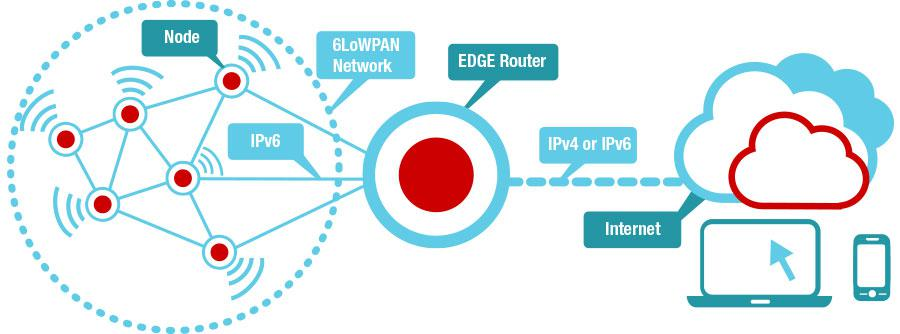
\includegraphics[width=16cm]{images/6lowpan.jpg}
	\caption{Diagramme d'explication de 6LoWPAN.}
	\label{fig:diagramme-6lowpan}
\end{figure}
L'équipe de recherche proposant ce sujet est le groupe 2XS \textbf{eXtra Small eXtra Safe} composée de notamment \textbf{Gilles GRIMAUD} notre encadrant, \textbf{Michael HAUSPIE} son collègue proche de ce sujet et bien sûr le reste de l'équipe.
L'équipe se focalise sur les problématiques de sécurité dans les systèmes embarqués contraints, notamment fournir des solutions logicielles prouvées.

%%% Local Variables: 
%%% mode: latex
%%% TeX-master: "isae-report-template"
%%% End: 
